\section{Alloy Model}

In this chapter the critical and most complex parts of the system are analyzed though Alloy model.\\
In particular the analysis focuses on the following components of the system: 
\begin{itemize}
    \item Discussion Forum
    \item Daily Plan
    \item Help Request (with related responses)
\end{itemize} \\
In the following model, these components are described specifying properties and constraints to validate the consistency of the corresponding generated worlds.\\
Some signatures and facts have been introduced or simplified in order to build the model, improving readability without losing accuracy.


\subsection{Signatures}

Vuoto
\subsection{Facts}

Vuoto
\subsection{Assertions}

Vuoto
\subsection{Analysis Results}

Vuoto
\subsection{Generated Worlds}

In this section are shown the three different Generated Worlds, one for each component analyzed through Alloy.\\

\lstinputlisting[language=alloy]{./Chapters/Chapter4/AlloySourceCode/Predicates.als}

\begin{figure}[H]
  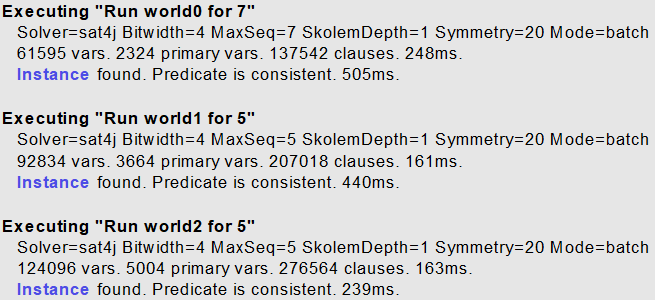
\includegraphics[width=\textwidth,height=\textheight,keepaspectratio]{./Images/Alloy/predicatesExecution.png}
  \caption{Alloy Analysis Results}
\end{figure}

\newpage
\KOMAoptions{paper=landscape,pagesize}
\recalctypearea
\begin{center}
\begin{sidewaysfigure}[H]
    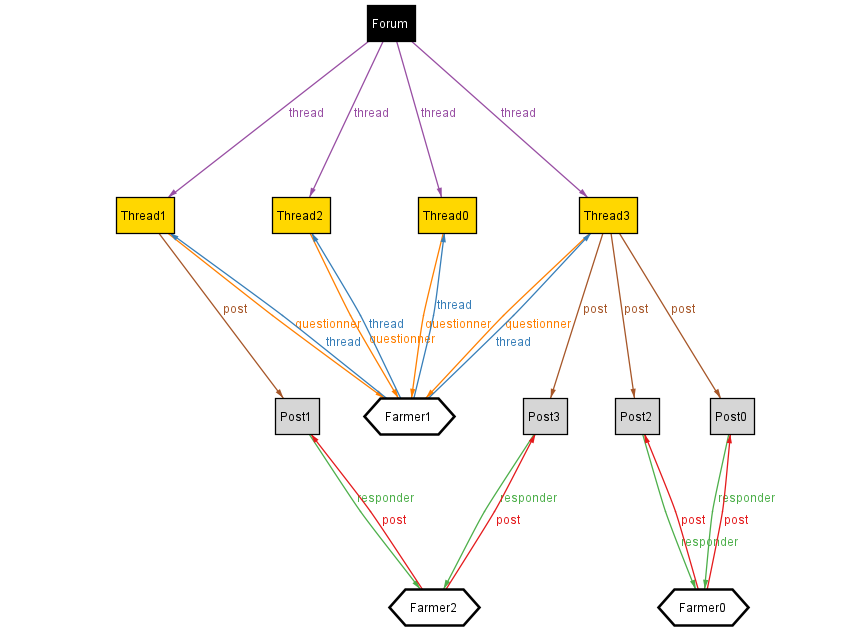
\includegraphics[width=\textwidth]{./Images/Alloy/DiscussionForum.png}
    \caption{Generated World0 - Discussion Forum}
    \label{fig:LandscapeFigure}
\end{sidewaysfigure}
\end{center}

\newpage
\KOMAoptions{paper=landscape,pagesize}
\recalctypearea
\begin{center}
\begin{figure}[H]
\centering
  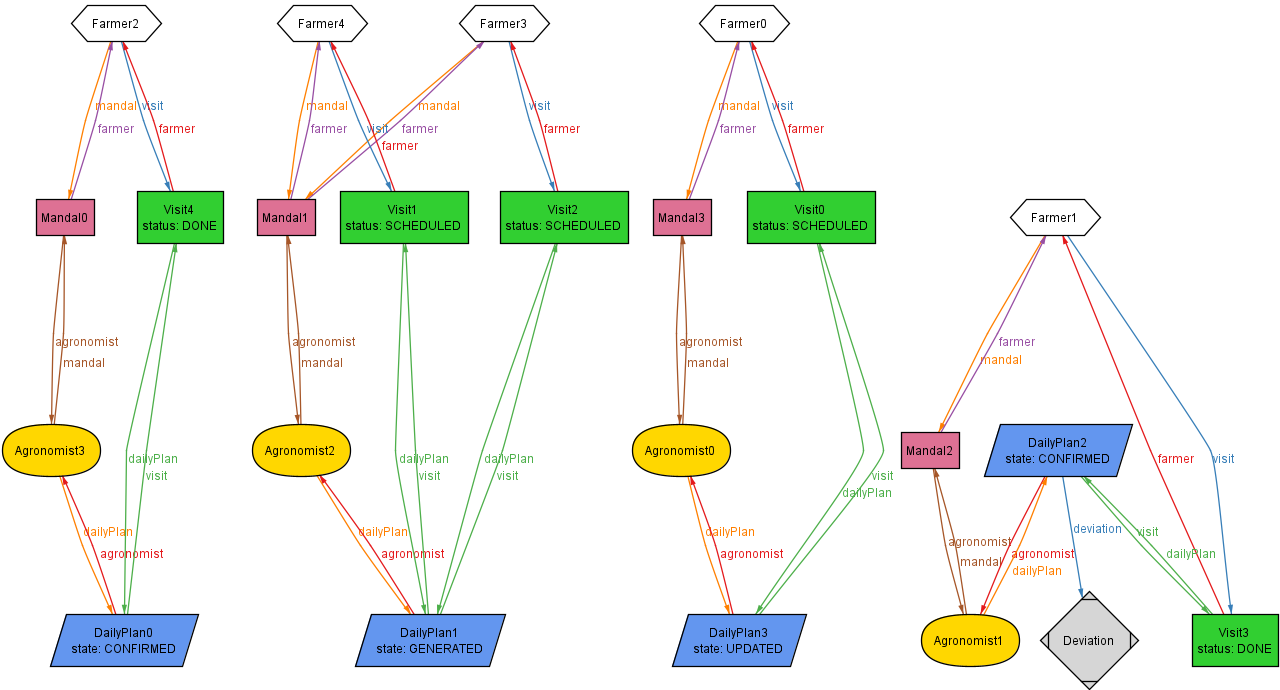
\includegraphics[angle = 90,scale= 0.4]{./Images/Alloy/DailyPlan.png}
  \caption{Generated World1 - Daily Plan}
    \label{fig:LandscapeFigure}
\end{figure}
\end{center}

\newpage
\KOMAoptions{paper=landscape,pagesize}
\recalctypearea
\begin{center}
\begin{figure}[H]
\centering
  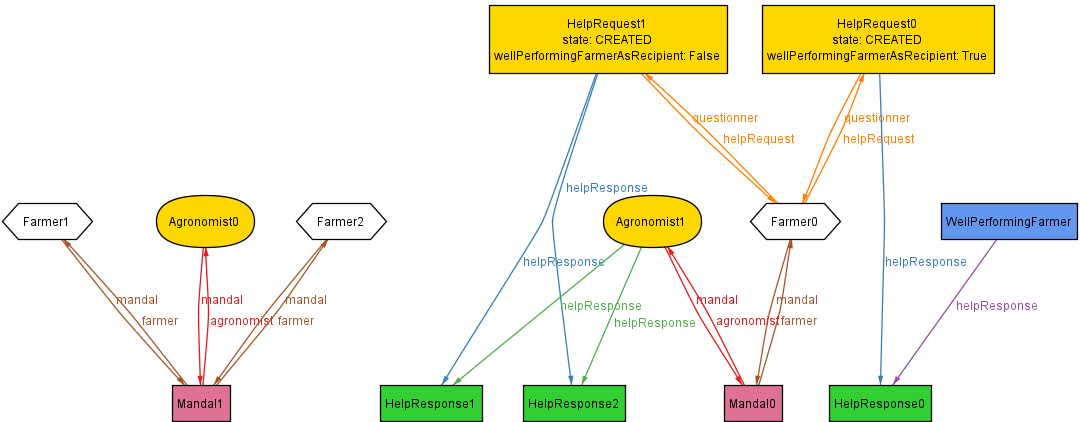
\includegraphics[angle=90,scale= 0.5]{./Images/Alloy/HelpRequest.png}
  \caption{Generated World2 - Help Request}
    \label{fig:LandscapeFigure}
\end{figure}
\end{center}

